%==========================================================================

\begin{frame}[fragile]

  {\Huge Backend Updates}

  \vspace{10pt}

\end{frame}


%==========================================================================

% Examples

% note: always keep the [fragile] for your frames!

%\begin{frame}[fragile]{Title}
%  Contents
%\end{frame}

%==========================================================================
\begin{frame}[fragile]{CUDA and SYCL}
  \begin{itemize}
    \item CUDA: Add support for AMPERE87 architecture (Jetson Orin Nano)
    \item CUDA: Support RDC with Clang 17+ and use new offload driver
    \item SYCL: Add support for Intel DG2 GPUs such as the Arc Alchemist GPUs
    \item SYCL: Allow using non-trivially-copyable comparators with oneDPL
  \end{itemize}
\end{frame}

%==========================================================================

\begin{frame}[fragile]{Improve half float performance for CUDA and SYCL backends}
  \begin{itemize}
    \item CUDA AND SYCL: Directly use the available fp16 mathematical function instead of casting back and forth to fp32
  \end{itemize}
  \begin{tikzpicture}
    \begin{axis}[
        width  = 0.85*\textwidth,
        height = 0.75*\textheight,
        major x tick style = transparent,
        ybar=2*\pgflinewidth,
        bar width=14pt,
        ymajorgrids = true,
        ylabel = {Exec time (µs)},
        symbolic x coords={Memory Bound Kernel, Compute Bound Kernel},
        xtick = data,
        scaled y ticks = false,
        enlarge x limits=0.25,
        ymin=0,
        legend style={at={(0.3,0.75)},anchor=west},
    ]
        \addplot
            coordinates {(Memory Bound Kernel, 32) (Compute Bound Kernel, 102)};

        \addplot
            coordinates {(Memory Bound Kernel, 15.8) (Compute Bound Kernel, 102)};

        \addplot
            coordinates {(Memory Bound Kernel, 14.7) (Compute Bound Kernel, 63)};

        \legend{float 32, fp16 old, fp16 new}
    \end{axis}
\end{tikzpicture}
\end{frame}

% Bench details:
% - NVidia A100
% - 2^20 (1 million) elements
% - Memory bound kernel is doing:
% tmp = init(i);
% res(i) = sqrt(cos(tmp) + sin(tmp));
% - Compute bound is doing 16 time the work of Memory Bound

%==========================================================================

\begin{frame}[fragile]{OpenMPTarget}
  \begin{itemize}
      \item Remove support for non-llvm compilers as part of the strategy to only support LLVM compilers in the backend.
      \item LLVM compilers support extensions to OpenMP directives on GPU that allow \textit{grid} style kernel launches making it more suitable for GPUs and avoiding the overhead of OpenMP's fork-join model.
  \end{itemize}
\end{frame}

%==========================================================================
